% grab the definitions for the PCN lab class
% 
\input{00_preamble}

% for this lab class.
\title{Demo -- FSL / UNIX}
\author{Denis Schluppeck} % {Denis Schluppeck}
\date{}                                           % Activate to display a given date or no date

\newcommand{\lab}{1}
\newcommand{\cmd}{\texttt{cmd}}


\begin{document}
\maketitle


\section{Setting up the computers -- everyone with their own login!}
This only needs to happen once to make sure the environment on your machines is set up correctly for when you next log on. Once you have done this, everything should work on consecutive logins (and in all the different computer labs). 

\begin{enumerate}

	\item Find the \unix{Terminal} application in the \folder{/Applications/Utilities/} folder and start it

	\item \textbf{I highly recommend:} start working through the overview of the Unix tutorial (read Introduction and Tutorial 1). You should be able to run each of the steps, although the screengrabs will look a little bit different as we are not running the same Unix/Linux, \url{http://www.ee.surrey.ac.uk/Teaching/Unix/}
	
	\item Find \folder{/Volumes/practicals/ds1} and look for the little robot guy with the label \textbf{Set Up My Machine}. \textbf{Double-click} and wait for a second.
%:Automator action
	\begin{center}
	\includegraphics[height=4cm]{automatoricon.png}	
	\end{center}
	
	You should see a message in a \textbf{dialog prompt} that looks as follows: 	
%: Automator dialog prompt
	\begin{center}
	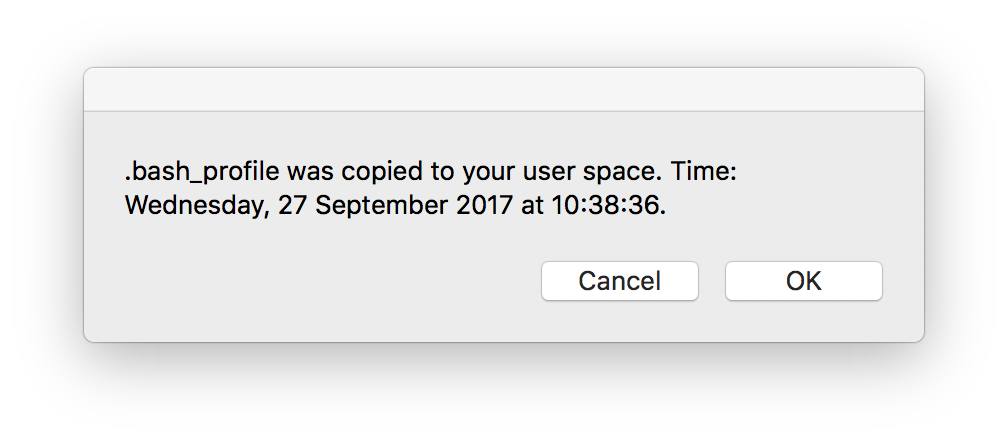
\includegraphics[height=4cm]{path-message.png}	
	\end{center}
	
	
	\item Now open a new Terminalwindow (\cmd-W closes the current window, \cmd-N opens a new one). You should now see some additional lines of text in the terminal window that read: \unix{[ ran custom .bash\_profile ]}  and \unix{Running FSL version: 5.0.4}. If you see this, then the setting up of your machine is done. Every time you log in from now and start the \unix{Terminal} application you'll be able to use the software straight away.
	
	\item Go to  \url{file:///Applications/Utilities} and start the program called \unix{XQuartz}. In theory, this should be launched automatically when you run the command in step \ref{runFSL}, but launching it by hand and enabling \emph{Start at Login} speeds things up a bit.
	
%:Xquartz screengrab
	\begin{center}
	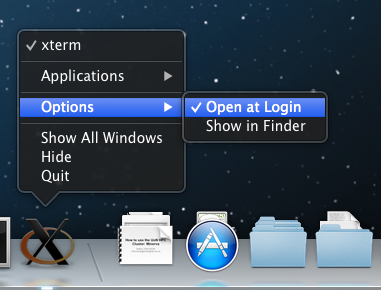
\includegraphics[width=8cm]{startXquartz.png}
	\end{center}

	\item Use the \unix{man} command (manual) to find out about three basic commands. \unix{cp} (copy), \unix{ls} (list) and \unix{more} (for looking at text files). Use the space-bar to go to the next page of the help documents and \unix{q} to quit the help.
	
\begin{lstlisting}[caption=Finding help for commands]
man ls # things behind a "#" are comments
man cp # this is the man-page for the Unix copy command
man more 
man cp 
\end{lstlisting}

\item Run the \unix{fsl} program from the command line
and start fslview with \unix{fsl \&} (the last button on the window that pops up on your screen).\label{runFSL} Alternatively, you can run the viewer program directly from the command line:  \unix{fslview \&}

%:FSL screengrab
	\begin{center}
	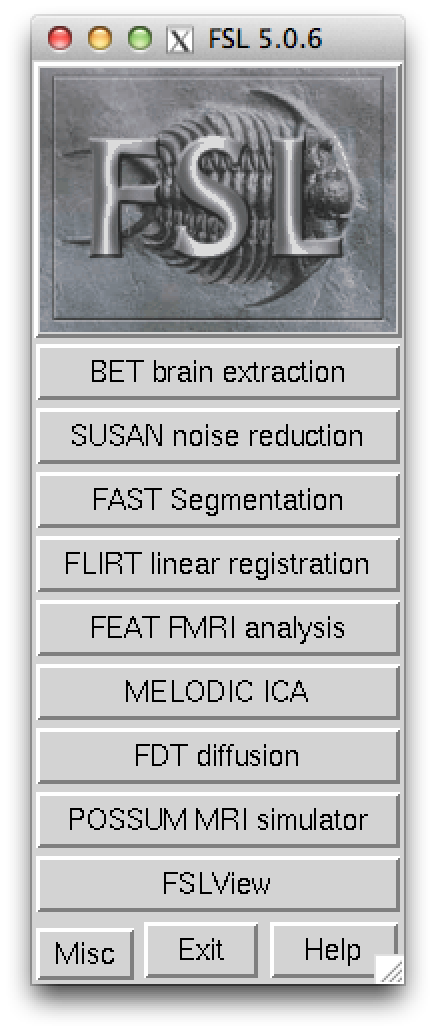
\includegraphics[height=9cm]{FSL-01.png}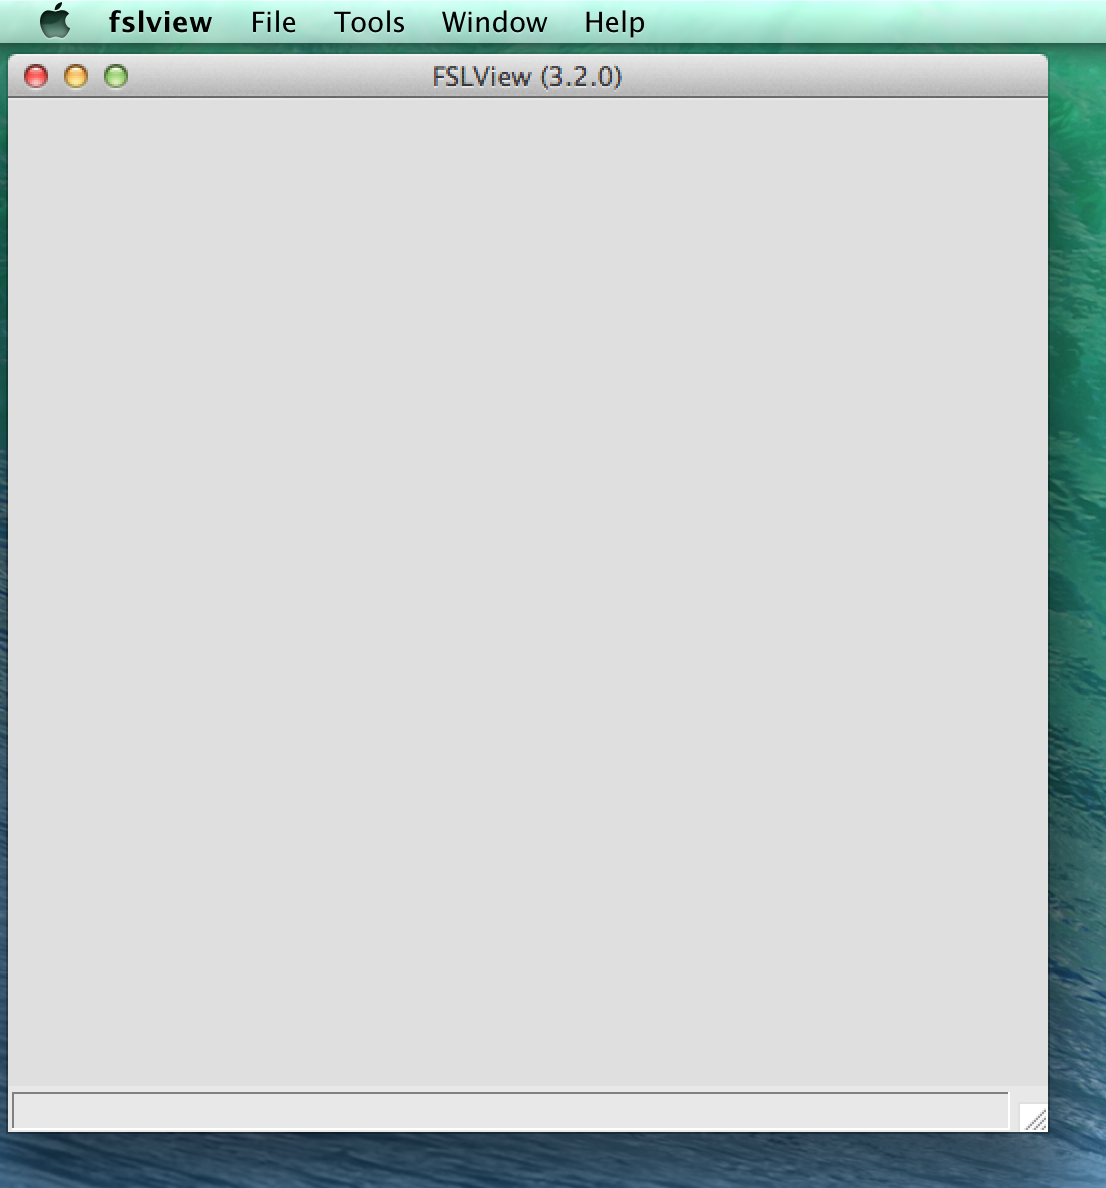
\includegraphics[height=9cm]{FSLview.png}

	\end{center}

\item File $\rightarrow$ Open Standard\dots\xspace and pick the file called \file{avg152T1.nii.gz} (or one of the other anatomy files in that folder, if you feel adventurous, noting down which one!)

% \item File $\rightarrow$ Open and using the \cmd-shift-and-G key, go to \url{file:///Volumes/practicals/ds1/data/anatomy} and pick one of the anatomy files.

\item Familiarize yourself with the viewer program. Help $\rightarrow$ Manual

\end{enumerate}



\section{A simple statistical analysis using FSL / FEAT}

\subsection{Overview}
In today's workshop, you'll see how to perform a complete statistical analysis as is done for real experiments. The data set we'll use is part of the materials of an FSL course organized by the FMRIB Centre at Oxford University. It was obtained in a language experiment, in which the subject was presented with 3 different \emph{events}. 

\begin{enumerate}
\item \emph{Word-generation} (WG), for which the subject was presented with a noun (e.g. water) and had to \emph{generate} an associated verb (e.g. boil, drink) and ``think of it''
\item \emph{Word-shadowing} (WS), for which the subject had to ``think of'' the presented word (but not generate anything)
\item \emph{Null events} (NULL), during which the fixation cross just remained and nothing happened. This is an important control condition that allows people to estimate the \emph{baseline} level of response.
\end{enumerate}

Rather than having \emph{blocks} that lasted 15-30s (as is often done in fMRI), each of these trials lasts 6s and they happen in (pseudo-)random order, e.g. something like
WS\dots WG \dots WG \dots NULL \dots WS \dots NULL \dots NULL \dots

The aim of the analysis is to work out which areas of the brain were more active during word generation and word shadowing than at rest, and which areas were more active in one condition rather than the other. We'll also look at a specific, pre-defined area (Broca's area in the left hemisphere) to see what the level of activity was in each of the conditions.

\subsection{Running the analysis}

I suggest you work through the following in your groups and discuss to make sure everyone in your group understands each step. To run the analysis, start up \unix{Feat\_gui} in the Terminal.

\begin{enumerate}

%: open feat
\item  \textbf{You should already have a copy of the data set in your \file{fslData} directory}, so there should be no need to do this first step again. If not, copy the data set from the network drive to a folder in your home directory, make the new folder your \emph{current working directory} by \unix{cd}'ing into it and start the program window for the main analysis program.

\begin{lstlisting}
# check if the fslData folder exists!  
# It shouldn't, as you've never done this before
ls ~/fslData 

# if not, copy the files
cp -r /Volumes/practicals/ds1/msc/fslData  ~/

# change directory to make it the "working directory"
cd ~/fslData

# and start FEAT. The & frees the Terminal up
Feat_gui &
\end{lstlisting}

\begin{center}
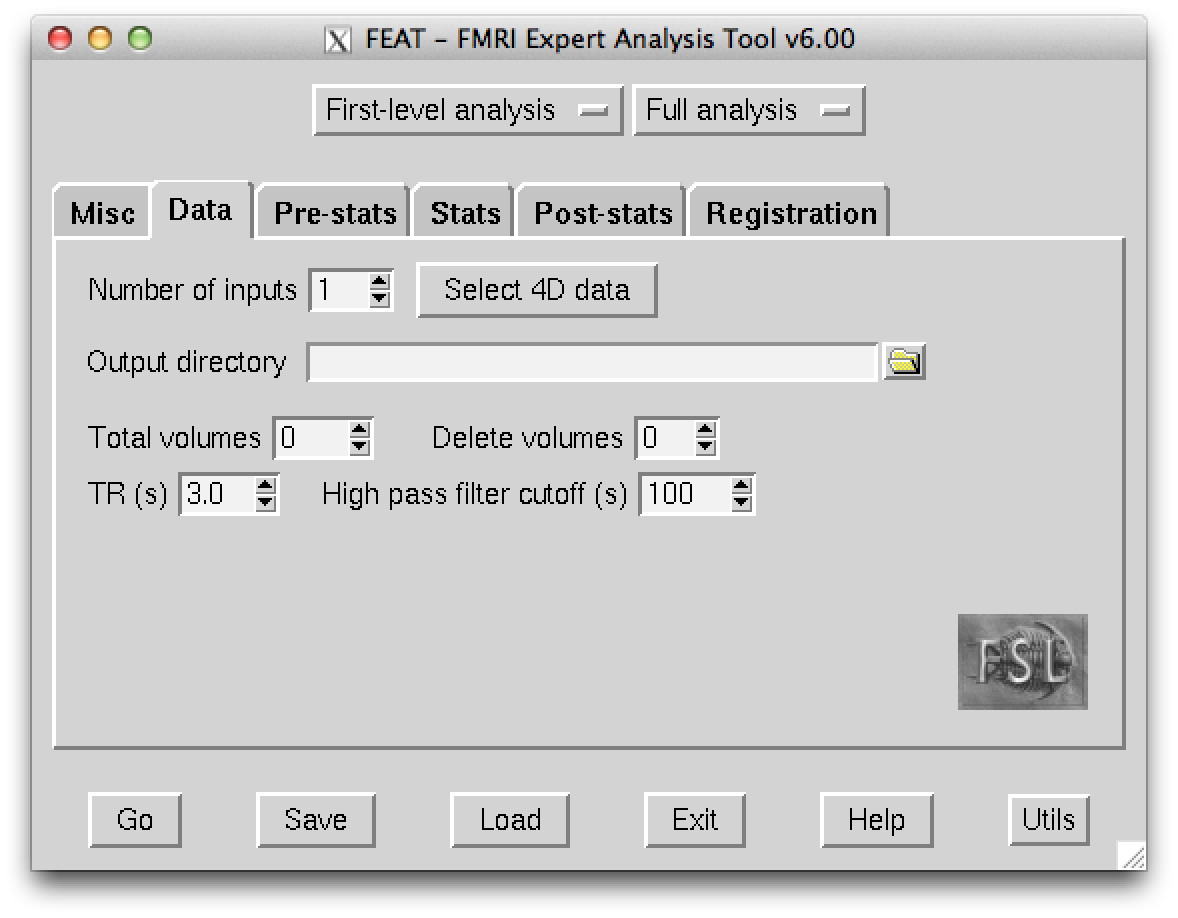
\includegraphics[width=7.5cm]{FEAT-snapshot.png}
\end{center}

%: open feat
\item The program opens up, automatically set to \emph{First-level analysis} and \emph{Full analysis}. There are several window tabs ("Data", "Pre-stats", \dots) and we need to step through each of them, to change a small number of settings.

\item In the \textbf{Data} tab: Click the \unix{Select 4D data} button and select the \unix{fmri.nii.gz} file by pressing the little folder icon in the pop-up window (note, that the file name will be different from what's shown in the screen shot here):

\begin{center}
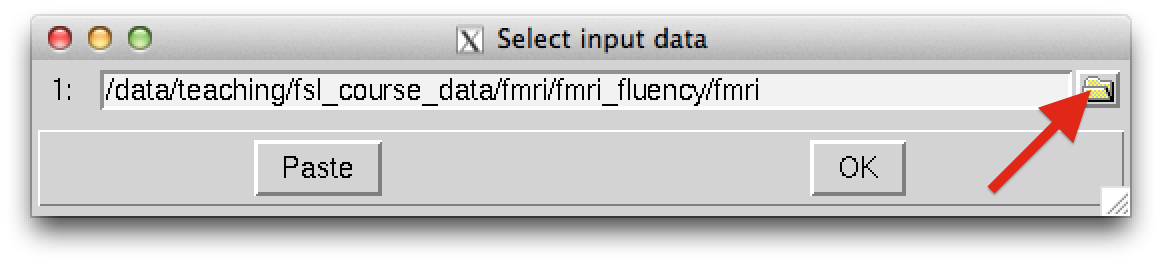
\includegraphics[width=7.5cm]{feat-4d-data.png}
\end{center}

\item You should now see the "Total volumes" field update to 106 and "TR (s)" to 4.2

\item In the \textbf{Pre-stats} tab: nothing to change. The defaults should work fine.

\item In the \textbf{Stats} tab: here we need to set up the \emph{model}, i.e. the timing of the different events that happened in the experiment. Click the \unix{Full model setup} button and do the following:

    \begin{itemize}
    \item "Number of original EVs" \textbf{2}. This creates two sub-tabs in the "EVs" part of the window.
    \item then for tab  \textbf{1}: "EV name" \textbf{generation}, "Basic shape"  \textbf{Custom (3 column format)} and select the \unix{word\_generation.txt} file, "Convolution"  \textbf{Double-Gramma HRF}
     \item then for tab  \textbf{2}: "EV name" \textbf{shadowing}, "Basic shape"  \textbf{Custom (3 column format)} and select the \unix{word\_shadowing.txt} file, "Convolution"  \textbf{Double-Gramma HRF}
     
     \begin{center}
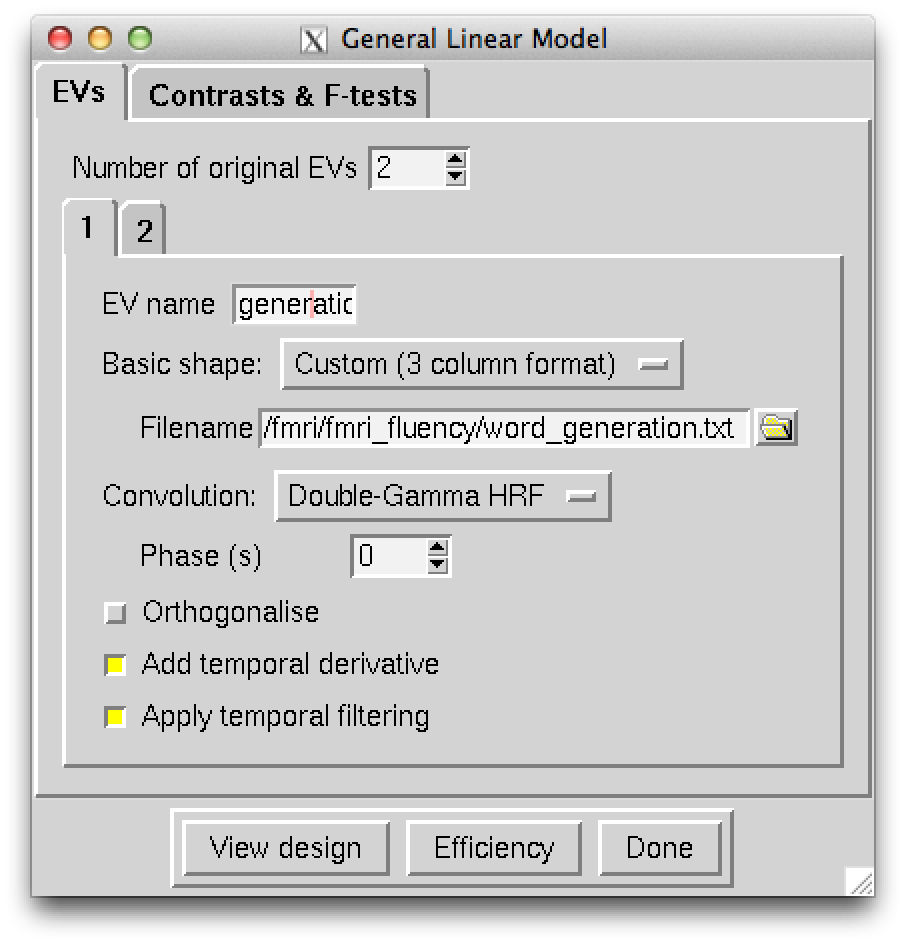
\includegraphics[width=7.5cm]{feat-evs.png}
	\end{center}
    
      \item In the "Contrasts \& F-tests" tab you can then set up \textbf{5 contrast} and \textbf{1 F-test}, entering text and clicking the up/down arrows until you have the following 5 contrasts\dots
   
\begin{center}
\begin{tabular}{lc}
Generation & [1 0] \\ 
Shadowing &  [0 1] \\ 
Mean & [1 1] \\ 
Shadow > Gen & [-1 1] \\ 
Gen > Shadow & [1 -1] \\  
\end{tabular}
\end{center}
    
     \begin{center}
    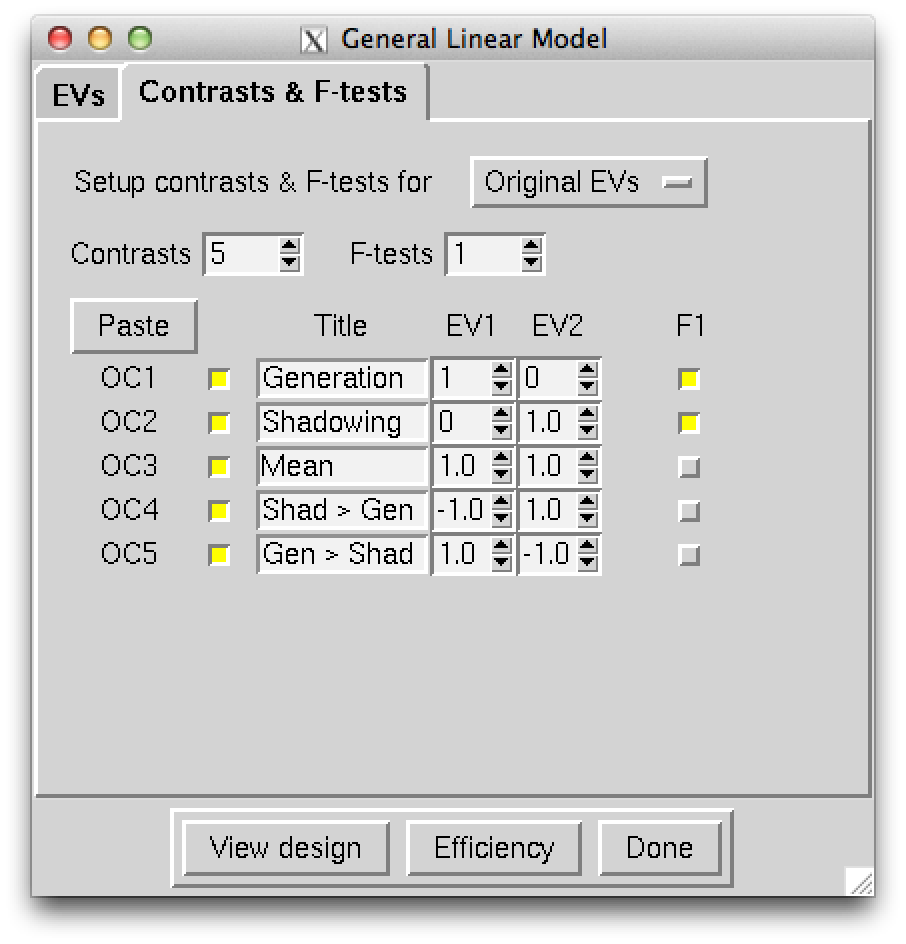
\includegraphics[width=7.5cm]{feat-contrasts.png}
	\end{center}
    
    \item If you know click the "View Design" button, you should see a window as follows (you may have noted that there are 4 columns, rather than 2. That's ok - the program has added two extra columns to deal with some slack in timing - this is a bit technical, but I am happy to explain if you are interested):
    
         \begin{center}
		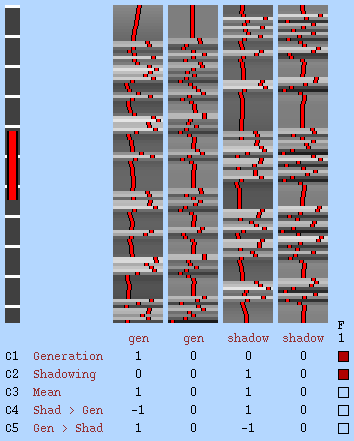
\includegraphics[width=7.5cm]{design.png}
	\end{center}
    
    \item Click "Done" and move on to the next tab.
    
      
    \end{itemize}

  \item In the \textbf{Post-stats} tab: nothing to change. The defaults should work fine.
    
    \item In the "Registration" tab, we need to do one more thing. Click on "Main structural image", and after clicking the folder button, you can select the \unix{structural\_brain.nii.gz} image to be used as an intermediate step in registration. \textbf{Important:} switch from the "BBR" method in the pulldown menu to the "7 DOF" one.
    
    \item Now we are done setting everything up. If you now press the \unix{Go} button, the analysis will start and a web browser should pop up and keep you posted on progress - how cool is this?
    
    \item \textbf{What do all those results mean?} We'll go through this in some detail next time. 
        
    The file \textcolor{red}{\unix{rendered\_thresh\_zfstat1.png}} is inside the folder that was created during the analysis, \unix{fmri.feat} by default. This image, note it's the one called \underline{\unix{z}}\unix{fstat}, shows areas that are more active during either word generation or shadowing, so when subjects are engaged in language processing.
    
    It should look something like the following:
    
         \begin{center}
    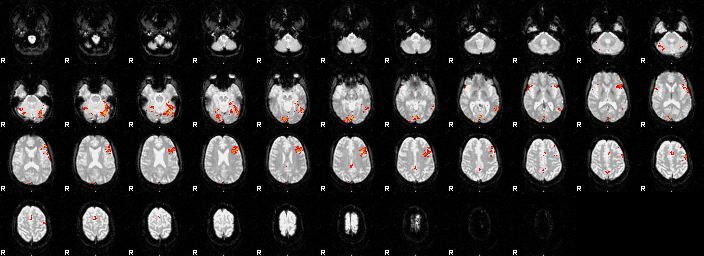
\includegraphics[width=13cm]{rendered_thresh_zfstat1.png}
	\end{center}
	
	\dots and if we zoom in, we can see a nice hotspot right around where we think Broca's area is:
	
	         \begin{center}
    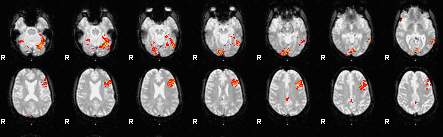
\includegraphics[width=13cm]{rendered_thresh_zfstat1_crop.png}
	\end{center}
	
	
\end{enumerate}

\hrule


\section{Questions}

\begin{itemize}
\item[A]	Use the \unix{man} command to get help about \unix{ls} . 
\item[B] What option would you use to get the \unix{ls} command to list things in the long format?
\item[C] What was the meaning of the special symbols tilde (\unix{\~}), hash \unix{\#}, the dot (\unix{.}) and the double-dot (\unix{..}); what was the point of the ampersand (\unix{\&}) ? Check back to \url{http://www.ee.surrey.ac.uk/Teaching/Unix/} if you have forgotten.

\vspace{.2cm}
\scalebox{1.0}{
	\begin{tabular}{|p{2cm}|p{4cm}|}
	\hline
	\textbf{symbol} & \textbf{means what?} \\
	\hline
	\unix{\~} & \\
	\hline
	\unix{\#} & \\
	\hline
	\unix{.} & \\
	\hline
	\unix{..} & \\
	\hline
	\unix{\&} & \\
	\hline
	\end{tabular}
}

\item[D]	Find out what the FSL command line tools \unix{fslinfo},  \unix{fslnvols}, and  \unix{slicer} do. 

\item[E]  Using some options with \unix{fslstats}, work out what proportion of voxels in the image \file{Broca.nii} are labelled (non-zero). How much is this in units of of voxels and mm$^3$? 

\item What is the volume of the cube that contains the image data of \file{Broca.nii}? Is there an option in \unix{fslstats} that can give you this answer? How could you work this out from "first principles"?

\end{itemize}

\hrule

\section{Ninja skills - Unix and FSL}

\begin{enumerate}

\item Make a directory called \file{workshopNotes} in your home directory using Unix commands in the terminal. Note down how you did it.

\item The Mac operating system has a command called \unix{say}. Check out what the following command call does
\begin{lstlisting}
say "This class rocks" 
\end{lstlisting}

\item What other options for this command can you find with \unix{man say}? Page all the way down to the EXAMPLES section of the man-page.

\item Have a look at the \emph{mask} (or \emph{region of interest}) I have pre-made for you. It's an image that labels all the voxels where we think there is a higher than 50\% probability of being in Broca's area in the left hemisphere (Brodmann areas 44 and 45, L).

\begin{small}
\begin{lstlisting}
fslview $FSLDIR/data/standard/MNI152_T1_2mm -l Greyscale Broca -l Red &
\end{lstlisting}
\end{small}

If you want to understand how this command works and pops up both images in different colormaps, have a look at the help for the \unix{fslview} program as follows:

\begin{lstlisting}
fslview --help
\end{lstlisting}

\item You can \emph{redirect} the output of the \unix{UNIX} commands into a simple text file. The redirect operator  (\unix{$>$}) does exactly what you want. For example, to put some text into a new text file you can use:

\begin{lstlisting}
echo "This is so cool."
# prints or "echo"s things in the Terminal

echo "This is so cool." > newTextFile.txt
# prints or "echo"s things into a new file 
# (and also creates it if needed)

ls newTextFile.txt

# and use the following to look inside the new file
cat newTextFile.txt

echo "My login is $LOGNAME" >> newTextFile.txt
# >> appends, the variable $LOGNAME contains your login!
\end{lstlisting}

\item Automatically copy the output of the command to the \emph{clipboard} (where you copy \& paste from usually in, say, Microsoft Word:

\begin{lstlisting}
fslmeants -i fmri -c 42 42 26 | pbcopy
# the | symbol represents a "pipe" and forwards
# the output to another command (rather than a text file)

#check out what pbpaste returns.
pbpaste 
\end{lstlisting}


\end{enumerate}

\section{Additional resources}
Check out information on the GLM (General[ized] Linear Model and various other statistical issues here):

\begin{itemize}
% \item Sample data set was obtained from \url{https://openfmri.org/dataset/ds000105}
\item \url{http://fsl.fmrib.ox.ac.uk/fslcourse/} 
\item \url{http://fsl.fmrib.ox.ac.uk/fslcourse/lectures/feat1_part1.pdf}
\end{itemize}

\end{document}  



